This chapter evaluates the testing methodology presented in this thesis, by
deriving testers from specifications and running them against systems under
test.  

I conduct the experiments on two kinds of systems, \http server
(\autoref{sec:http}) and file synchronizer (\autoref{sec:sync}).  The research
questions are: (1) Qualitative: Can the tester find invalid behavior from the
SUT? and (2) Quantitative: How long does it take the tester to reveal invalid
behavior?

\section{Testing Web Servers}
\label{sec:http}

This thesis is motivated by the Deep Specification project~\cite{deepspec},
whose goal is to build systems with rigorous guarantee of functional
correctness, studying HTTP as an example.  I formalized a subset of \http
specification, featuring WebDAV requests GET, PUT, and POST~\cite{rfc4918}, ETag
preconditions~\cite{rfc7232}, and forward proxying~\cite{rfc7231}.

From the protocol specification written as ITrees, I derived a tester client
that sends and receives network packets.  \autoref{sec:http-sut} explains the
system under test and the experiment setup.  \autoref{sec:http-qual} and
\autoref{sec:http-quant} then describe the evaluation results qualitatively and
quantitatively.

\subsection{Systems Under Test}
\label{sec:http-sut}
I ran the derived tester against three server implementations:

\begin{itemize}
\item Apache HTTP Server~\cite{Apache}, which is among the most popular servers
  on the World Wide Web~\cite{http-netcraft,http-stats}.  I used the latest
  release 2.4.46, and edited its configuration file to enable WebDAV and proxy
  modules.
\item Nginx~\cite{nginx}, the other most popular server.  The experiment was
  conducted on the latest release 1.19.10, with WebDAV and proxy modules enabled
  separately, because they cannot work together as Apache does.
\item A simple web server developed in C by \citet{itp21}, supporting GET and
  POST requests.  The server's functional correctness was formally verified.  We
  aimed at developing formal specifications that are testable and verifiable.
\end{itemize}

The tests were performed on a laptop computer (with Intel Core i7 CPU at 3.1
GHz, 16GB LPDDR3 memory at 2133MHz, and macOS 10.15.7).  The Apache and Nginx
servers were deployed as Docker instances, using the same host machine as the
tester runs on.  Our simple server was compiled into an executable binary, and
also ran on localhost.

The tester communicates with the server via POSIX system calls, in the same way
as over Internet except using address \inlinec{127.0.0.1}.  The round-trip time
(RTT) of local loopback is $0.08\pm0.04$ microsecond (at 90\% confidence).

\subsection{Qualitative Result}
\label{sec:http-qual}
\paragraph{Apache}
My tester rejected the Apache HTTP Server, which uses strong comparison for PUT
requests conditioned over \inlinec{If-None-Match}, while RFC~7232 specified that
\inlinec{If-None-Match} preconditions must be evaluated with weak comparison.
\bcp{What are strong and weak comparison?  \lys{ETag jargons.}}  I reported this
bug to the developers, and figured out that Apache was conforming with an
obsoleted \http standard~\cite{rfc2616}.  The latest standard has changed the
semantics of \inlinec{If-None-Match} preconditions, but Apache didn't update the
logic correspondingly.

\lys{Under construction:}

We created 20 mutants by manually modifying the Apache source code.  The tester
rejected all the 20 mutants, located in various modules of the Apache server:
\inlinec{core}, \inlinec{http}, \inlinec{dav}, and \inlinec{proxy}.  They appear
both in control flow ({\it e.g.}, early return, skipped condition) and in data
values ({\it e.g.}, wrong arguments, flip bit, buffer off by one byte).

We didn't use automatic mutant generators because (i) Existing tools could not
mutate all modules we're interested in; and (ii) The automatically generated
mutants could not cause semantic violations against our protocol specification.

When testing Nginx, we found that the server did not check the preconditions of
PUT requests.  We then browsed the Nginx bug tracker and found a similar ticket
opened by \citet{nginx242}.  These results show that our tester is capable of
finding bugs in server implementations, including those we're unaware of.
%% \bcp{But you just described a known bug!}

\subsection{Quantitative Result}
\label{sec:http-quant}

\begin{figure*}
  
\includegraphics[width=\textwidth]{figures/http-time}
  \caption[Cost of detecting bug in each server/mutant]{Cost of detecting bug in
    each server/mutant.  The left box with median line is the tester's execution
    time before rejecting the server, which includes interacting with the server
    and checking its responses.  The right bar with median circle is the number
    of \http messages sent and received by the tester before finding the bug.
    Results beyond 25\%--75\% are covered by whiskers.
    %% \bcp{The red horizontal
    %%   lines are very confusing: make them blue!  Also, we need to explain
    %%   what all the parts of the figure mean (or, better, remove most of
    %%   them!)---the thin dotted parts, thin solid parts, why the dotted ones
    %%   are terminated and the solid ones are not, ...}
  }
  \label{fig:checker-performance}
\end{figure*}

As shown in \autoref{fig:checker-performance}, the tester rejected all buggy
implementations within 1 minute.  In most cases, the tester could find the bug
within 1 second.

Some bugs took longer time to find, and they usually required more interactions
to reveal.  This may be caused by (1) The counter-example has a certain pattern
that our generator didn't optimize for, or (2) The tester did produce a
counter-example, but failed to reject the wrong behavior.  We determine the real
cause by analysing the bugs and their counterexamples:

\begin{itemize}
  \begin{figure}
    \lys{Duplicates with \autoref{fig:reordered-trace} and
      \autoref{fig:invalid-trace}.}
    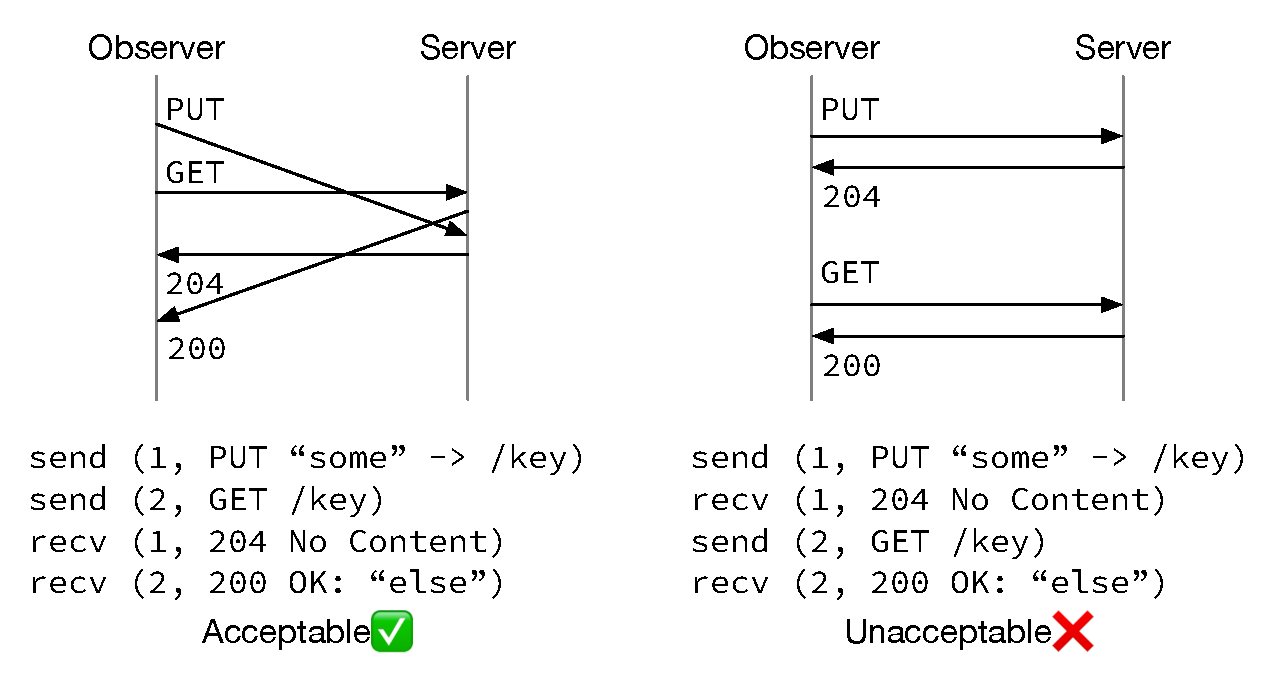
\includegraphics[width=\linewidth]{figures/http-put-bug}
    \caption{The trace on the left does not convince the tester that the server
      is buggy, because there exists a certain network delay that explains why
      the PUT request was not reflected in the 200 response.  When the trace is
      ordered as shown on the right, the tester cannot imagine any network
      reordering that causes such observation, thus must reject the server.}
    \label{fig:put-bug}
  \end{figure}
  \item Mutants 19 and 20 are related to the WebDAV module, which handles PUT
    requests that modify the target's contents.  The buggy servers wrote to a
    different target from that requested, but responds a successful status to
    the client.  The tester cannot tell that the server is faulty until it
    queries the target's latest contents and observes an unexpected value.  To
    reject the server with full confidence, these observations must be made in a
    certain order, as shown in \autoref{fig:put-bug}.

  \item Mutant 18 is similar to the bug in vanilla Apache: the server should have
    responded with 304 Not Modified, but sent back 200 OK instead.  To reveal
    such violation, a minimal counterexample consists of 4 messages: (1) GET
    request, (2) 200 OK response with some ETag \inlinec{x}, (3) GET request
    conditioned over \inlinec{If-None-Match: x}, and (4) 200 OK response,
    indicating that the ETag \inlinec{x} did not match itself.  Notice that (2) must be
    observed before (3), otherwise the tester will not reject the server, with a
    similar reason as \autoref{fig:put-bug}.

  \item Mutant 5 causes the server to skip some code in the core module, and
    send nonscence messages when it should respond with 404 Not Found.  The
    counterexample can be as small as one GET request on a non-existential
    target, followed by a non-404, non-200 response.  However, our tester
    generates request targets within a small range, so the requests' targets are
    likely to be created by the tester's previous PUT requests.  Narrowing the
    range of test case generation might improve the performance in
    aforementioned Mutants 18--20, but Mutant 5 shows that it could
    also degrade the performance of finding some bugs.

  \item The mutants in proxy module caused the server to forward wrong requests
    or responses.  When the origin server part of the tester accepts a
    connection from the proxy, it does not know for which client the proxy is
    forwarding requests.  Therefore, the tester needs to check the requests sent
    by all clients, and make sure none of them matches the incoming proxy
    request, before rejecting the proxy.
\end{itemize}

These examples show that the time-consuming issue of some mutants are likely
caused by limitations in the test case generators.  Cases like Mutant 5 can be
optimized by tuning the request generator based on the tester model's runtime
state, but for Mutants 18--20, the requests should be sent at
specific time periods so that the resulting trace is unacceptable per
specification.  How to produce a specific order of messages is to be explored in
future work.

\section{File synchronizer}
\label{sec:sync}
